\documentclass[11pt,a4paper]{article}
\usepackage[margin=0.5in]{geometry}
\usepackage{listings}
\usepackage[utf8]{inputenc}
\usepackage[english]{babel}
\usepackage{amsmath}
\usepackage{amsfonts}
\usepackage{amssymb}
\usepackage{graphicx}
\usepackage{enumerate}
\usepackage{color}
\usepackage{algorithm}

\usepackage{arydshln}

\setlength{\dashlinedash}{0.2pt}
\setlength{\dashlinegap}{4.5pt}
\setlength{\arrayrulewidth}{0.2pt}
\title{\bf BIOSTAT 615 Final Project\\
Reduced Rank Envelope Regression }  % Supply information
\author{Yixi Li, Sunghun Lee, Pedro Orozco del Pino\\
https://github.com/shnlee-ds/Rpackage-Reduced\_Rank\_Envelope\_Regression}              %   for the title page.
\date{December 14, 2018}      
\begin{document}
\maketitle                              
%\flushleft \textbf{BIOSTAT 615 Final Project}\\
%Reduced Rank Envelope Regression\\
%Yixi Li, Sunghun Lee \& Pedro Orozco del Pino\\
%Due December 14, 2018\\
\section{Introduction}
\subsection{Background}
The multivariate regression model is the following:
$$Y=\beta X+\epsilon,$$
where $Y\in \mathbb{R}^{r\times 1}$, $X\in\mathbb{R}^{p\times 1}$, $\beta\in\mathbb{R}^{r\times p}$
In multivariate regression analysis there is the case in which the coefficients matrix is not full rank. In such cases the reduced-rank methodology can get a better estimate than OLS. Another improvement that can be done in multivariate analysis is when the estimation of the beta matrix can be done with less information without compromissing accuracy. For this, we look a subspace in which the projection of the response is immaterial of the covariates. This means that the kernel projection of the response is independent of the projection given the covariates and also is independent of the covariates. The envelope regression methodology estimates this subspace and also outperforms OLS. Each of this methodologies is an improvement of OLS multivariate regression that could be combined. In this project we build a program that combines reduced-rank and envelope regression methodologies into an R package. Each of the methodologies don't compite with each other since they attain different challenges. The reduced-rank envelope regression combines strenghts of each of the methodologies and it doesn't amplifies weaknes, it is because of this that the combine methodology outperforms OLS, reduced-rank and envelopes. 



\subsection{Envelopes Regression}

The envelope model tries to estimate the smallest subspace $\mathcal{E} \subseteq \mathbb{R}^u$, (u$\leq$r) such that

$$Q_{\mathcal{E}}Y	|X\sim Q_{\mathcal{E}}Y,\quad\quad cov(Q_{\mathcal{E}}Y,P_{\mathcal{E}}Y|X)=0$$
This means that we are looking for a subspace in which $Q_{\mathcal{E}}Y$ is linearly immaterial to the estimation of $\beta$ in the sense that it responds neither to changes in the predictor nor to those in the rest of response. 
The dimension u of $\mathcal{E}$ is going to be one important parameter in our discussion.
\subsection{Reduced Rank Regression}
The reduced-rank regression allows $rank(\beta)=d\leq\min (r,p)$. Under some well studied constraints on the parametrization of $\beta=AB$, $A\in \mathbb{R}^{r\times d}$, $B\in \mathbb{R}^{d\times p}$ with $rank(A)=rank(B)=d$ the MLE of the reduced-rank regression is:

$$\hat{\beta}_{RR}=S_Y^{1/2}C_{XY}^{(d)}S_X^{-1/2},\quad C_{XY}=S_Y^{-1/2}S_{XY}S_X^{-1/2},$$

where $X^{(d)}$ is the construction of matrix X with the d largest eigen values.
\subsection{Reduced Rank Envelope Regression}
Let $(\Gamma,\Gamma_0)$ be  an orthogonal basis for $\mathbb{R}^r$ so that span($\Gamma)$ is the projection of $\beta$ into $\mathcal{E}$ and $\Gamma\in\mathbb{R}^{r\times u}$ then:

\begin{equation}\label{eq:rre}
\beta=\Gamma\eta B,\quad \Sigma=\Gamma\Omega\Gamma^T+\Gamma_0\Omega_0\Gamma_0^T,
\end{equation}
where $\Omega\in\mathbb{R}^{u\times u},\Omega_0\in\mathbb{R}^{(r-u)\times (r-u)}$ are symmetric positive definite matrix and $\eta$ carries the coordinates of A with respect to $\Gamma$. 
Under the Gaussian error model the likelihood of $\beta$ is a multivariate normal.
Hence, the likelihood $L_n(\eta,B,\Omega,\Omega_0,\Gamma|d,u)$ is:

\begin{align}\label{eq:likelihood}
-\frac{n}{2}\left\lbrace log|\Sigma(\Gamma(u),\Omega(u))|+
\frac{1}{n}\sum\limits_{i=1}^n\left(Y_i-\Gamma(u)\eta(u,d) B(d)X\right)\Sigma(\Gamma(u),\Omega(u))\left(Y_i-\alpha-\Gamma(u)\eta(u,d) B(d)X\right)^T\right\rbrace
\end{align}
where $\Sigma(\Gamma,\Omega)=\Gamma\Omega\Gamma^T+\Gamma_0\Omega_0\Gamma_0^T$ also as functions of u but we omit them.
The maximum likelihood then is:
\begin{equation}\label{eq:MLE}
\hat{\beta}_{RE}=\hat{\Gamma}S_{\hat{\Gamma}^TY}^{1/2}C_{X\hat{\Gamma}^TY}^{(d)}S_X^{-1/2}
\end{equation}

When u=r, this is equivalent to set $\Gamma=I_r$ and \ref{eq:MLE} is the same as the reduced-rank estimator. On the other hand, if d=p then \ref{eq:MLE} is the same as in the only envelope model.
\section{Methods}
\subsection{Implementation of reduced-rank envelope regression}
The pseudocode of the implementation of reduced-rank envelope regression is as follows:\\
\vspace{0.1cm}\\
\textbf{Data: multivariate data (X,Y), with dimension of X is p$\times$N, and dimension of Y is r$\times$N}\\
\textbf{Output: Return the best selection of (u,d), estimates of beta, fitted values, residuals, variance of residuals, error table}
\begin{enumerate}
\item if (u,d) is not given, do:
\begin{enumerate}
\item select (u,d) by rrenv.choose\_du(X, Y, Beta=NULL)
\item return the best selection of (u,d)
\end{enumerate}
\item if (u,d) is given, do:
\begin{enumerate}
\item check whether the input (u,d) is valid
\end{enumerate}
\item reduced-rank envelope regression:
\begin{enumerate}
\item envelope estimation:
\begin{enumerate}
\item estimate the envelope by envlp(X,Y,u,d)
\item return Gamma, Gamma0
\end{enumerate}
\item reduced-rank regression
\begin{enumerate}
\item estimate beta by R\_reduced\_rank\_envelope\_given\_u\_d(X,Y,u,d, Gamma, Gamma0) in C++
\item return estimates of beta, fitted values, residuals, variance of residuals, error table
\end{enumerate}
\end{enumerate}
\end{enumerate}
Finally, the reduced-rank enevelope regression is implemented in R and C++, and is wrapped into a R package, rrenv.

An example of how to use rrenv is:
\begin{lstlisting}[language=R]
#input X and Y
Y<-as.matrix(read.table("Y.txt"))
X<-as.matrix(read.table("X.txt"))
est <- rrenv(X,Y,20,10,NULL)
#returns
beta<-est$beta
fit_values<-est$fit_values
residuals<-est$residuals
residual_variance<-est$residual_variance
error_table<-est$error_table
\end{lstlisting}

\subsection{Selection of parameter d and u}
A feature that the rrenv package has is a built in function that gives a suggestion for the choice of (u,d). 
This suggestion is based on exploring exhaustively the AIC for all combinations of (u,d). 
We choose to do this search exhaustively because as shown in the Figure \ref{fig:choose_du} right panel the AIC is very sensible to small variations in (u,d). 
It is open for improvement to optimize AIC with a more efficient algorithm, however that was out of the scope of this project.
The explicit formula of the AIC is:
\begin{equation}\label{eq:AIC}
AIC=2N_{RE}-2L_{u,d}=(p+r-d)d+r(r+1)/2-2L_{u,d},
\end{equation}

where $L_{u,d}$ is the likelihood of the model given (u,d). 
We also show in Figure \ref{fig:choose_du} that AIC replicates reasonably well the search of an optimal (u,d) by minimizing $||\hat{\beta}-\beta||_F$. 
In real scenarios we $\beta$ is of course unknown, however the package has also the option of input a true beta 
When you have a data, a function rrenv.choose\_du(X, Y, Beta=NULL) in our package recommends the combination of parameter (d, u) for a reduced-rank envelope regression modeling based on the error calculation. When you input the matrices of X, Y and the true Beta matrix(the left case of below figure), the function calculates $||\hat{\beta}-\beta||_F$,  while it calculates $AIC=2N_{RE}-2L_{u,d}=(p+r-d)d+r(r+1)/2-2L_{u,d}$
\begin{figure}
\centering
\label{fig:choose_du}
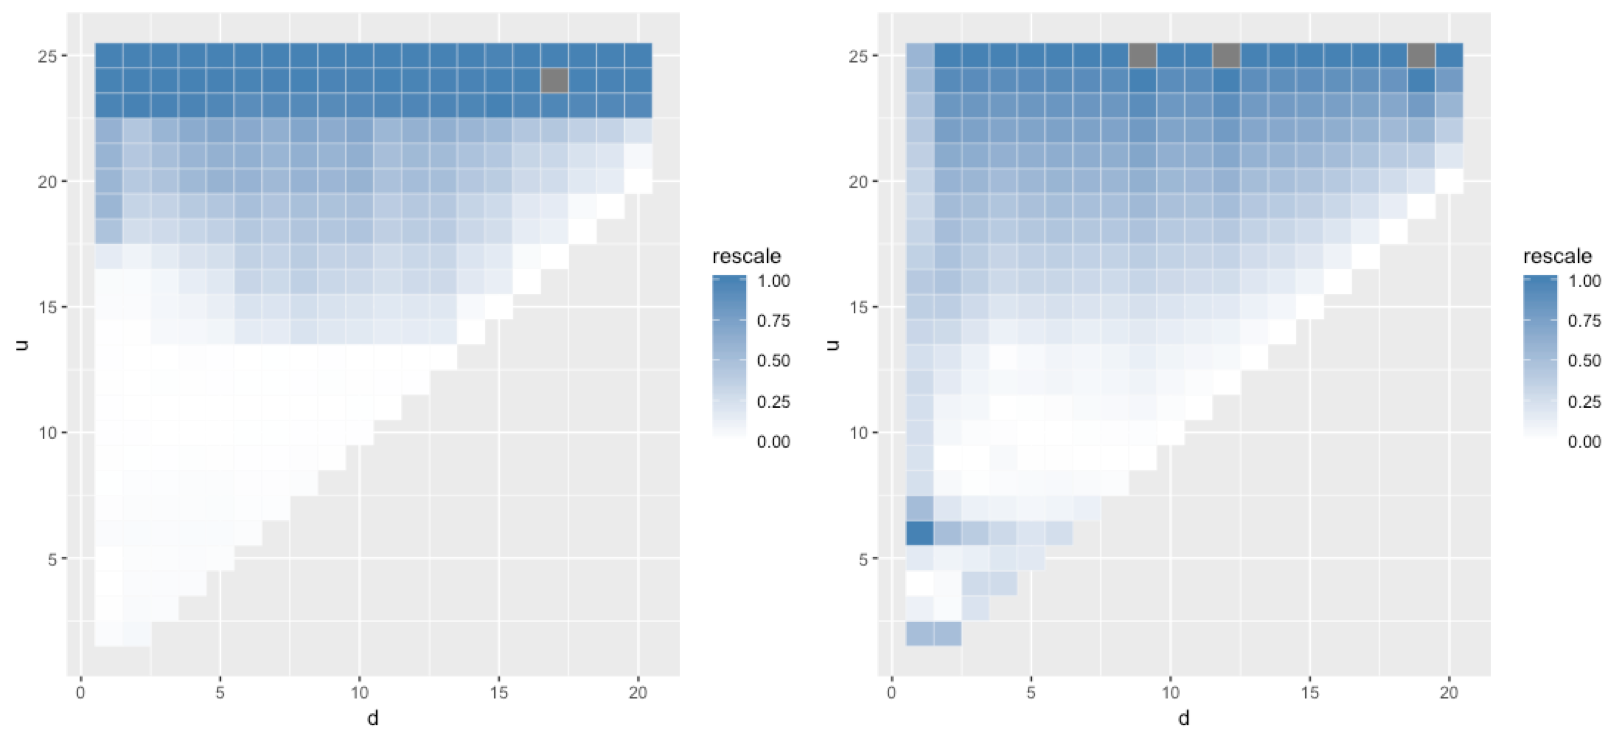
\includegraphics[scale=.6]{choose_du.png}
\caption{Left panel has the heat map of $||\hat{\beta}-\beta||_F$ when comparing with the true $\beta$. Right panel shows the AIC heatmap}
\end{figure}
\section{Simulations}
We compared the performance (in terms of the fit of model) of our new Reduced-rank envelope package and existing R packages (for OLS, Reduced-rank regression and Envelope regression). 
As you can see from Figure \ref{fig:accu}, the Reduced-rank envelope regression model with our new R package always showed the best performance in all the three cases.
\begin{figure}
\centering
\label{fig:accu}
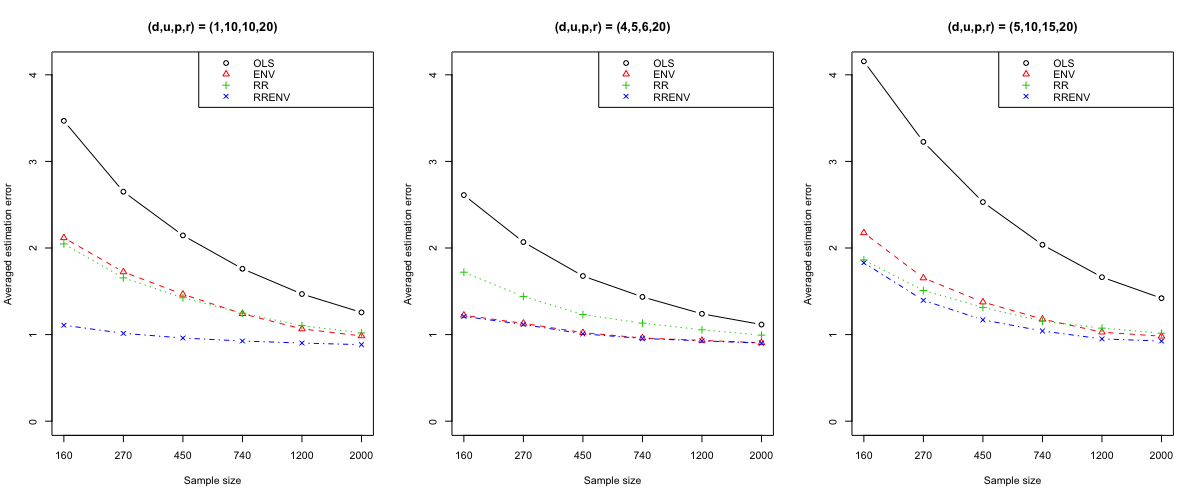
\includegraphics[scale=.4]{accuracy.png}
\caption{In the y axis $||\hat{\beta}-\beta||_F$, in the x axis is sample size (160, 240, 450, 740, 1200, 2000). }
\end{figure}
In addition, it is also impressive that Reduced-rank envelope was stable between different sample sizes from 160 to 2000. 
In particular, it is noteworthy that in a small sample size, its performance was superior to other methods. 
The first scenario (left most panel) is design to be ideal for reduced rank regression because the rank of the betas is only 1 and the envelope was the same as the amounts of predictions. 
For this case the RRE outperforms all three methodologies by almost one magnitude in small sample sizes. 
The second scenario shows that when the rank of beta matrix is close the dimension of the envelope the RRE gives a modest improvement over envelope regression. 
Lastly we show a case in which the reduce rank and the envelope methodologies by themselves should be useful. 
RRE still outperforms all of them in all of the sample sizes. 
The takeaway from this is that RRE adapts when one of the methodologies is not ideal and when they are combines them adequately. 
\begin{figure}
\centering
\label{fig:bench}
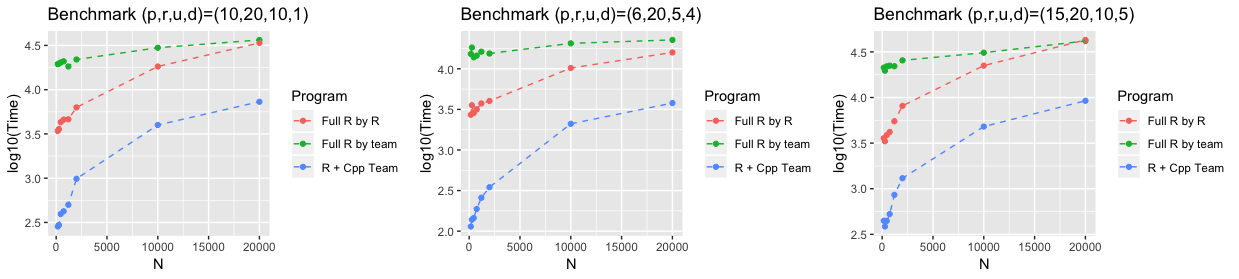
\includegraphics[scale=.42]{Benchmark.png}
\caption{Comparison of time of implementation of RRE in three ways. In red is by sequentially using two R libraries, in green an implementation made by the team all in R and finally in blue implementing the reduce rank part in C++. The panels are different combinations of parameters for the simulation, on the x axis is sample size (160, 470, 740, 1200, 2000,10000,20000) and log base 10 time in the y axis.}
\end{figure}
\newpage
\section{Discussion}

The RRE regression is a useful technique to address the multivariate regression problem.
The challenges that faces is that the MLE estimation is done under the space of subspaces of $\mathbb{R}^r$ (also call the Gransmannian).
However, a closed form for that was found by Cook (2015) and that simplifies the method.

The RRE depends highly matrix computations that is why we thought that a C++ implementation could be considerably faster than the existing packages of R. 
Even though it was expected to have an improvement in speed with a C++ implementation the simulations shown in Figure \ref{fig:bench} exceeded them.
The rrenv package is at least 10 times faster than sequentially using the two libraries of R and a little more than that that our own implementation on R.
Since we compared our own algorithm made in R and C++ Figure \ref{fig:bench} not only means that each of the libraries of R (env and rrr) can be improved with a C++ implementation but also confirms the superiority of C++ in matrix computations.

The R package rrenv also improves the accuracy of estimation in comparison to using only  an envelope or a reduced-rank model. 
This is not surprising since Cook (2015) showed that in the article this project is based on.
The downside is that this efficient estimation is conditional on knowing (u,d) which rrenv does have a implementation to get a good suggestion of (u,d) but is not computationally efficient.
As future work a better optimization of (\ref{eq:AIC}) could be done by many methods. 
The challenge of doing this is that (\ref{eq:likelihood}) has a very complicated form as a function of (u,d).

Finally the rrenv returns as well useful information to do further analysis like an estimation of $\Sigma$, fitted values and residuals.
Because of lack of time we didn't implemented any statistical test for significance.
If this should be done in the future we suggest a bootstrap approach since the variance of $\hat{\beta}$ is complicated even under the Gaussian assumption.


\begin{thebibliography}{999}

\bibitem{Cook}
  R.Dennis Cook, Liliana Forzani, Xin Zhang
  \emph{\LaTeX: Envelopes and reduced-rank regression}.
  Biometrika,  Volume 102, Issue 2, 1 June 2015, Pages 439–456

\end{thebibliography}

\end{document}